\chapter{Results}\label{chap:res}
Our system is able to produce biologically relevant dimensionality reductions that allow us to make better reduce models for \gls{cfps} systems.
We show the following key points:
\begin{itemize}
\item \gls{pca} and naive \glspl{vae} cannot learn good representations of different models, while our Corr-VAE can.
\item The separation between the different models improves as we add more latent dimensions.
This is replicated across different \gls{cfps} systems.
\item As noise is added to our model, Corr-VAE performance falls off, showing that we are learning real trends in the data.
\item We can use the latent representations of our Corr-VAE to reduce \glspl{gem} and create \gls{cfps} models that correlate better with experimental data.
\end{itemize}

%TODO show that we're better than PCA

% Is VAE better than PCA?
% Need to use Corr-VAE in order to reconstruct space
% Noise/actually reconstructing space
% Reduction
% Biological insights
% Transfer learning

\section{Can a \gls{vae} distinguish between fluxes generated from different experimental conditions?}
We want to use our \gls{vae} to learn how changes in the experimental conditions affect the underlying \gls{cfps} system.
If the \gls{vae} is going to be useful for us to extract information about the underlying cell-free system, it will need to be able to distinguish between different starting experimental conditions.
In order to assess how well our \gls{vae} is learning the differences between experimental conditions, we can examine the latent space of the \gls{vae}.
If our \gls{vae} is performing well, we should see a clear separation between fluxes generated from different models.
For this set of experiments, we run on the set of fluxes generated from our manual dataset.
The \gls{pca} and regular \gls{vae} are trained on the flat version of the manual dataset, while our Corr-VAE is trained on the stacked version.
All three techniques project the same test dataset into 2 dimensions for visualization purposes.
The \gls{vae} and the Corr-VAE have identical networks of 3 layers of size 1024 for their encoder and decoder networks.

Figure \ref{fig:vae_pca} visualizes the latent space of a basic \gls{vae} as well as the first two principal components of the \gls{pca}.
Both dimensionality reduction techniques fail to uncover the underlying structure of the fluxes.
This demonstrates that naive applications of a \gls{vae} or \gls{pca} cannot learn the differences between the various starting experimental conditions.

\begin{figure}[t!]
\begin{center}
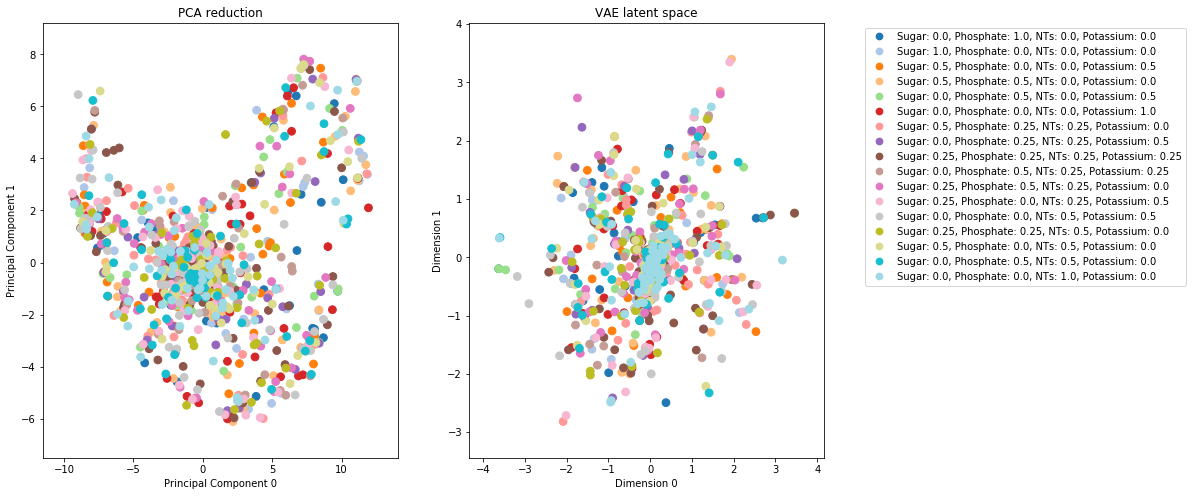
\includegraphics[width=1.2\textwidth]{figs/vae_vs_pca_latent.png}
\caption[Comparison of the latent dimensions \gls{pca} and \gls{vae}]{Left: first two principal components of a \gls{pca} on our test dataset.
Right: the two latent dimensions of a trained \gls{vae} with the classic loss function.
Different colors represent different experimental conditions.
Neither \gls{pca} nor a basic \gls{vae} can learn a clear representation of the different models we are using.}
\label{fig:vae_pca}
\end{center}
\end{figure}

However, when we use our custom loss function, we are able to recover clear distinctions between the different conditions.
Figure \ref{fig:corrvae_2d} plots the latent space of our Corr-VAE.
Whereas the experimental conditions cannot be recovered in the latent space of the \gls{vae}, the latent space of the Corr-VAE clearly distinguishes between the different starting conditions.
While \gls{pca} is a popular dimensionality reduction technique in biology, these results demonstrate that Corr-VAE may be a more effective way to understand data.

\begin{figure}[t!]
\begin{center}
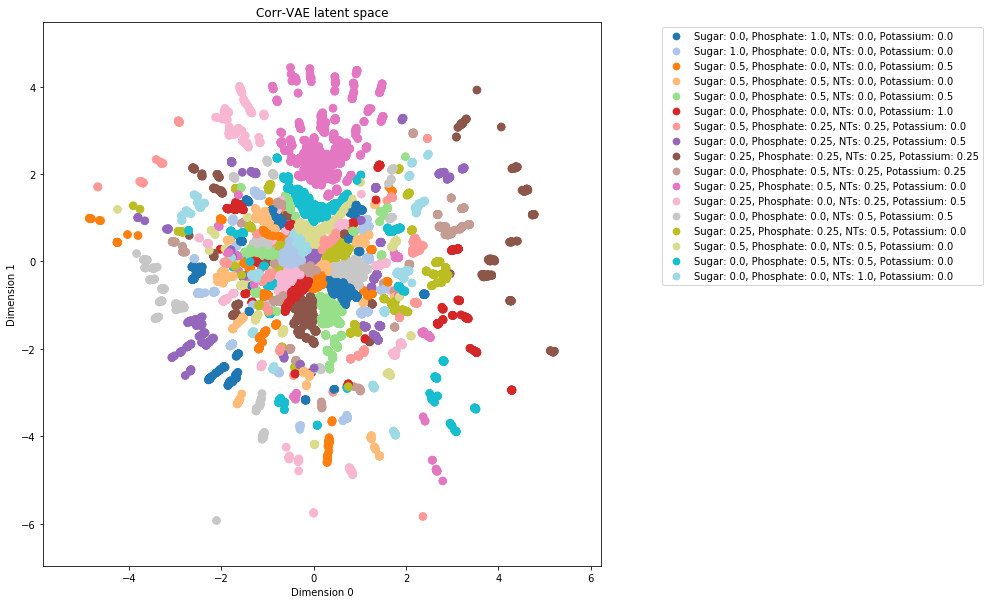
\includegraphics[width=1.01\textwidth]{figs/corrvae_hand_2d_latent.png}
\caption[Latent dimensions of our Corr-VAE network]{Different colors represent different experimental conditons.
This plot shows the two latent dimensions of a trained Corr-VAE.
Colors cluster together and show that a Corr-VAE can recover the original models.}
\label{fig:corrvae_2d}
\end{center}
\end{figure}

Our original dataset had on the order of 2600 features, so using a latent space of only 2 dimensions is a very severe dimensionality reduction.
We also trained a Corr-VAE with a latent space that had 10 dimensions to see if more dimensions allowed for better reconstruction.
In order to visualize the latent space of this Corr-VAE, we projected our 10-dimensional latent space down to 2 dimensions using the \gls{tsne} method~\cite{maaten2008visualizing}.
Figure \ref{fig:manual_10d} shows that using a 10-dimensional latent space with a Corr-VAE is able to clearly separate different starting experimental conditions.
These results suggest that more biological applications should consider using a \gls{vae} instead of \gls{pca} for dimensionality reduction purposes.
We also show that this technique can generalize across different \gls{cfps} systems.
Figure \ref{fig:karim_10d} is generated using the same structure for our Corr-VAE, but on the Karim dataset.

\begin{figure}[t!]
\begin{center}
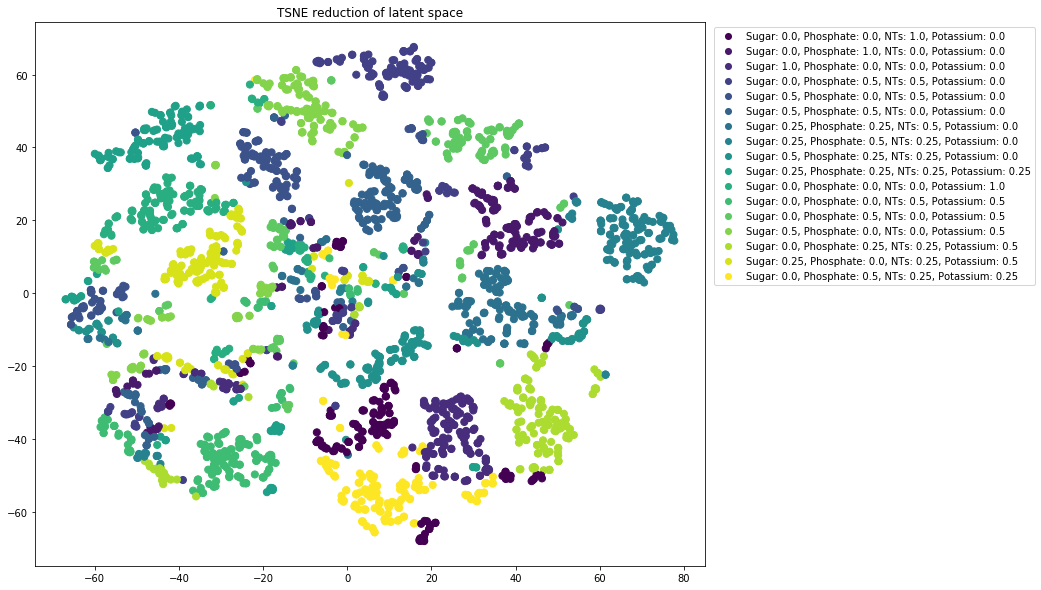
\includegraphics[width=1.01\textwidth]{figs/TSNE_hand_latent10.png}
\caption[Projection of the latent space of a 10-dimensional Corr-VAE trained on the Manual dataset]{Different colors represent different experimental conditons.
This plot shows a \gls{tsne} projection of the 10-dimensional latent space of a Corr-VAE trained on the Manual dataset.
Adding more latent dimensions allows better reconstruction of the invidual models.
}
\label{fig:manual_10d}
\end{center}
\end{figure}

\begin{figure}[t!]
\begin{center}
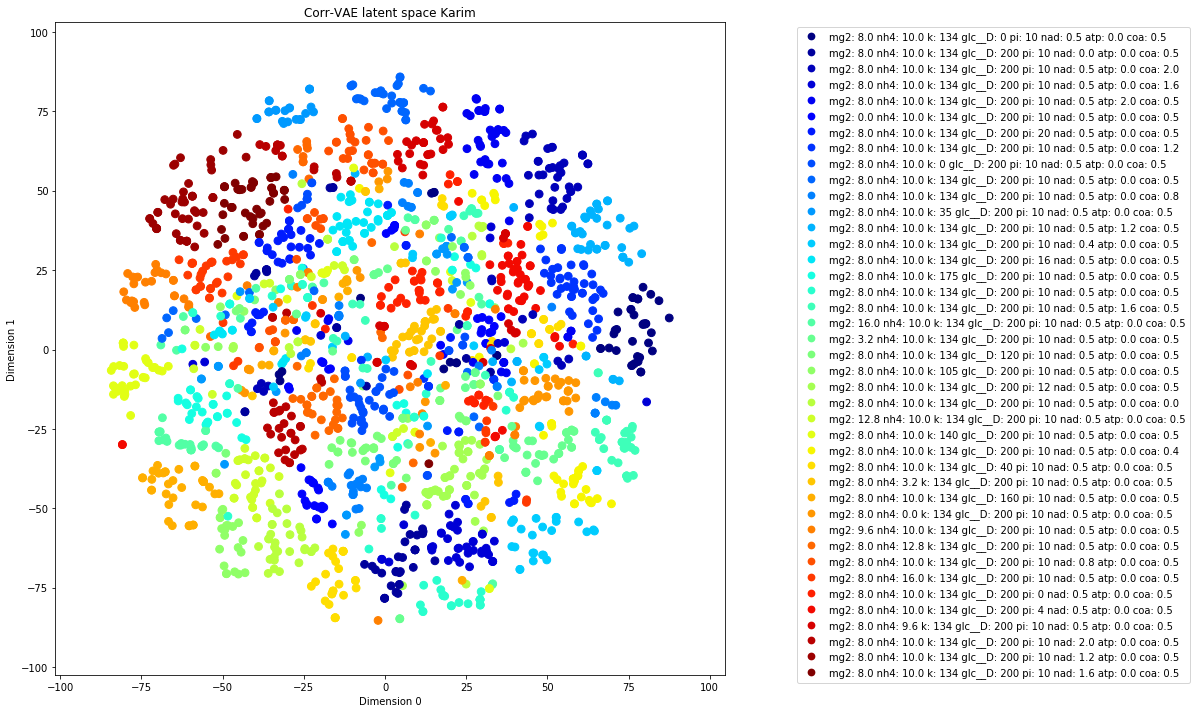
\includegraphics[width=1.01\textwidth]{figs/corrvae_karim_10d_latent.png}
\caption[Projection of the latent space of a 10-dimensional Corr-VAE trained on the Karim dataset]{Different colors represent different experimental conditons.
This plot shows a \gls{tsne} projection of the 10-dimensional latent space of a Corr-VAE trained on the Karim dataset.
Our Corr-VAE is able to reconstruct the individual models for multiple types of \gls{cfps} systems.
}
\label{fig:karim_10d}
\end{center}
\end{figure}

\section{Noise experiments}
We also validated that our \gls{vae} was performing as intended.
We can examine a few aspects of our reconstructed fluxes to ensure that the results we are seeing are not simply due to chance.
Figure \ref{fig:recon_stds} plots the standard deviations of each of the reactions for our test dataset as well as our reconstructed dataset.
We can see that the reconstructed dataset maintains a very similar shape to our original dataset, while also reducing the standard deviation of fluxes with each reaction.
Although we did not investigate this further, this implies that the \gls{vae} could also be used to de-noise our dataset.

\begin{figure}[t!]
\begin{center}
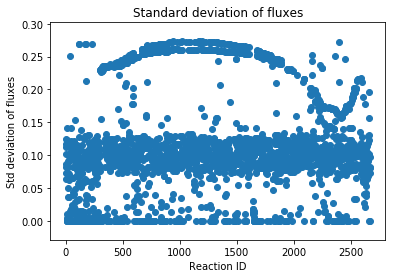
\includegraphics[width=1.01\textwidth]{figs/Reconstructed_stds.png}
\caption[Reconstructing fluxes reduces the amount of noise]{Reconstructed fluxes reduce the amount of noise while also maintaining the shape}
\label{fig:recon_stds}
\end{center}
\end{figure}

Another key point we investigated was whether or not the correlations we produce are spurious.
We wanted to ensure that our \gls{vae} is not creating correlations out of thin air just to reduce its loss function.
Figure \ref{fig:noise} shows what happens when we add noise to our experimental data.
First, we generate a dataset with fluxes that are highly correlated to our experimental data.
This is represented by the green line. 
We can then run those fluxes through our \gls{vae} and check the correlation.
The blue line shows that this improves the correlation of our fluxes because of our loss function.
Next, we can add noise to the data by randomly drawing from a normal distribution and adding it to the flux for each reaction.
The dots show that as we add increasing amounts of noise to the data, the correlation goes to about 0.
This means that the \gls{vae} is not simply artificially creating a correlation but is learning something about the underlying data.

\begin{figure}[t!]
\begin{center}
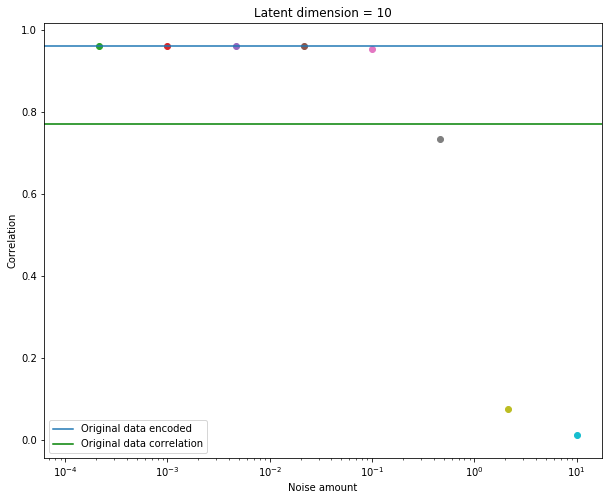
\includegraphics[width=1.01\textwidth]{figs/Noise_add.png}
\caption[Noise added to input data reduces the efficacy of a Corr-VAE]{Adding noise to the data reduces the correlation from our \gls{vae}}
\label{fig:noise}
\end{center}
\end{figure}

\section{Comparison of reduced models}\label{sec:cmp}
A key goal for our system was to produce reduced models that could accurately explain our biological data.
We tested this by solving for the optimal flux distribution for each model of our reaction conditions.
We then found the correlation between the predicted output and the real biological output.
Table \ref{tab:cmp} shows the results for each of our starting models that are at the \gls{gem} scale as well as some reduced models.
As expected, we found that the full-scale \glspl{gem} have very low correlations, between $0.14$ and $0.24$.
This models are intended to describe living \ecoli cells and thus do a poor job of modeling \gls{cfps} systems.

We also compare our model to pre-existing pruned models that other algorithms have created.
For instance, the ColiPruned model from NetworkReducer has a correlation of $0.34$ with our biological data.
This is better than the full-scale genome models, though it is not as good as our customized cell-free models.
This make sense because the goal of NetworkReducer is to reduce to a minimal core model, not to specify it for cell-free systems.
Our system produces models that with more than 2x better correlations than a full-scale \gls{gem}.
While these correlations show that we still cannot perfectly describe the biological system, the reduction is far better than a full-scale model.

\begin{table}[t]
\centering
\begin{tabular}{llll}
Dataset & TXTL & Reduced & Correlation \\
echo    & Yes   & No        & 0.22        \\
echo    & No    & No        & 0.14        \\
manual    & Yes    & No        &   0.23     \\
manual    & No   & No        &   0.24     \\
karim   & No    & No        & 0.17      \\
coli-pruned & No & Yes & 0.34 \\
manual-reduced & Yes & Yes & 0.50 \\
karim-reduced & Yes & Yes & 0.43 
\end{tabular}
\caption{Comparison of models.
Models that have been produced by our pipeline end in 'reduced'.
We compare the full \glspl{gem} to our reduced models and show that the using our system improves the correlation with real data}
\label{tab:cmp}
\end{table}

%\section{Biological Insights}
%TODO

%\section{Transfer learning}
%Another aspect that we were particularly interested in is how well the models would transfer between different experimental settings.
%TODO: write up and add figure